\chapter{Implementazione}
\label{ch:impl}

La figura \ref{fig:architettura-modify} mostra i nodi in linea tratteggiata che sono stati modificati per implementare la funzionalità nell'architettura di SeismoCloud:

\begin{itemize}
\item \textbf{API principali}: sono state implementate le API progettate nel capitolo precedente;
\item \textbf{MariaDB}: sono state create le tabelle necessarie in SQL basandosi sulla progettazione del capitolo precedente;
\item \textbf{Worker}: sono stati aggiunti dei compiti periodici che sono separati dalle API, e quindi dall'interazione diretta con i client;
\item \textbf{MinIO}: è stato aggiunto un \textit{bucket} per conservare le immagini associate ai messaggi. Un bucket è un modo di organizzare gli oggetti simili alle cartelle di un filesystem, ma è un termine specifico per un object storage server com'è MinIO.
\item \textbf{Nominatim}: sono state implementate delle interfacce per interagire con il servizio esterno Nominatim tramite le API pubbliche. Il servizio è utilizzato per l'assegnazione di un nome di una chat nelle API principali e per l'associazione di una chat con il terremoto in Worker.
\end{itemize}

\begin{figure}[ht!]
\centering
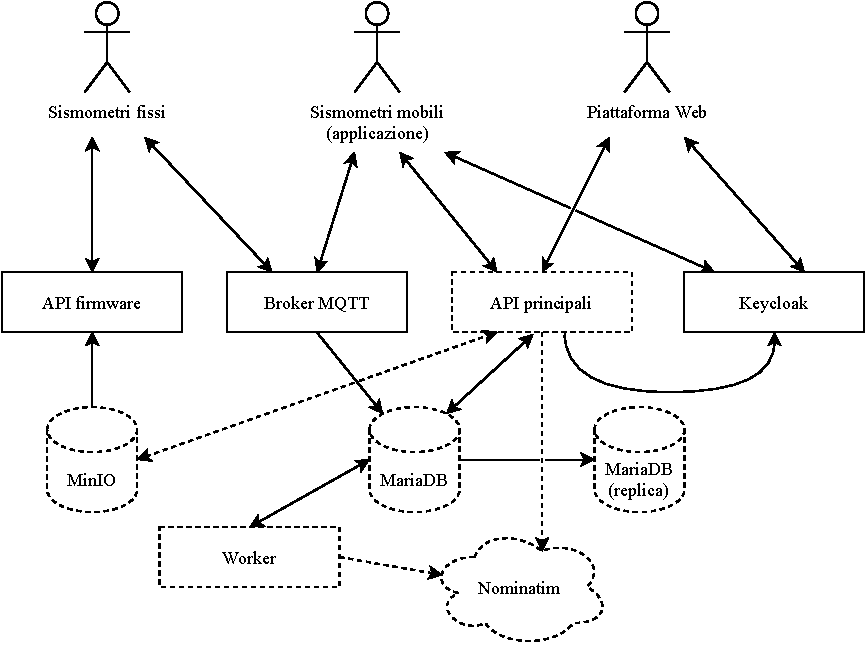
\includegraphics[width=\textwidth]{assets/04/architettura-modify.pdf}
\caption{Nodi coinvolti nell'implementazione della funzionalità.}
\label{fig:architettura-modify}
\end{figure}

Dal momento che MariaDB e MinIO sono software preesistenti, non hanno richiesto lavori di sviluppo poiché sono stati semplicemente configurati per la funzionalità. Lo sviluppo vero e proprio è invece avvenuto nelle API principali e nel Worker, due software realizzati in linguaggio Go. Per poter descrivere le sfide implementative e le scelte adottate durante il processo, è necessaria quindi una breve panoramica sul linguaggio e sull'organizzazione del codice backend di SeismoCloud.

\section{Il linguaggio Go}

\paragraph{Linguaggio Go} Go \cite{go}, il cui logo è mostrato nella figura \ref{fig:logo_go}, è un linguaggio di programmazione tipizzato staticamente e multi-paradigma, sintatticamente simile al C, che mira a una compilazione efficiente, un'esecuzione veloce e di una facile programmazione. Le due principali implementazioni sono un compilatore self-host, che prevede anche un insieme di strumenti per gestire un progetto in Go, e \texttt{gccgo}, la versione implementata per il compilatore GCC.

\begin{wrapfigure}{r}{0.30\textwidth}
\centering

\includegraphics[scale=0.20]{assets/04/logogo.png}
\caption{Logo di Go.}
\label{fig:logo_go}
\end{wrapfigure}

In Go è possibile programmare in paradigma orientato alla concorrenza, funzionale e imperativo, con una connotazione particolare per gli oggetti. Prevede dei meccanismi di sicurezza per la memoria, tra cui una gestione della memoria (\textit{garbage collection}, GC) e uno stile di concorrenza basato sullo scambio di messaggi attraverso dei canali. Il listato di codice \ref{listing:hello_world} mostra il classico programma dimostrativo in Go, che stampa un messaggio nell'output testuale. I principali utilizzi di Go sono per la costruzione di programmi che interagiscono con la rete o per programmi a riga di comando.

\paragraph{Go e SeismoCloud} In SeismoCloud Go è utilizzato per implementare le API esposte ai client e per i compiti periodici eseguiti in modo indipendente dalle API. Viene utilizzata l'ultima versione disponibile del linguaggio e della principale implementazione, la 1.16, che consiste in un compilatore e diversi strumenti aggiuntivi per la gestione del progetto.

\begin{listing}
\begin{minted}{go}
package main

import "fmt"

func main() {
	fmt.Println("Hello, World!")
}
\end{minted}
\caption{Classico programma dimostrativo ``Hello World!'' in Go.}
\label{listing:hello_world}
\end{listing}

\paragraph{Organizzazione del codice} Due concetti importanti in Go sono i \textit{moduli} e i \textit{package}. Un modulo è una collezione di package che sono sviluppati e distribuiti insieme, mentre un package è collezione di codici sorgenti in Go che risiedono nella stessa cartella. Un package può contenere a sua volta altri package. Il backend di SeismoCloud, d'ora in poi indicato solo con ``SeismoCloud'', è organizzato in una singola repository composta da un modulo e diversi package che suddividono il sistema in modo sia orizzontale che verticale. La figura \ref{fig:repository} mostra tale suddivisione. I package all'interno di \texttt{service} sono pensati per essere utilizzati in base alle necessità del singolo servizio. Un esempio è \textit{scsfilestorage}, responsabile dell'interazione con MinIO, utilizzato sia dalle API firmware che dalle API principali, nel primo caso per distribuire gli aggiornamenti ai firmware, nel secondo per distribuire le immagini. Invece quelli in \texttt{cmd} sono una suddivisione verticale, per cui \texttt{webapi} contiene il codice necessario per le API principali, mentre \texttt{worker} contiene il codice necessario per il Worker.

\begin{figure}[ht!]
\centering
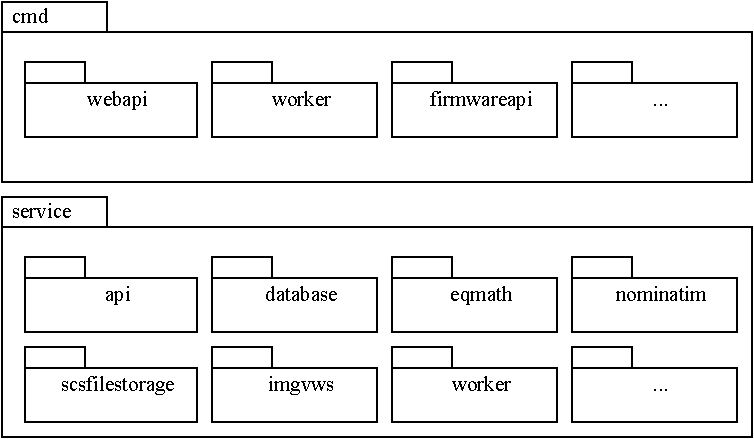
\includegraphics[width=0.8\textwidth]{assets/04/repository.pdf}
\caption{Organizzazione dei principali package di SeismoCloud.}
\label{fig:repository}
\end{figure}

\section{Implementazione delle API}

Una volta configurato il database, sono state implementate tutte le API progettate seguendo uno schema comune. I package principalmente coinvolti sono due:

\begin{itemize}
\item \texttt{api}: package che implementa tutte le api principali. Ognuna ha una file di codice sorgente associato, che contiene di solito la funzione principale che gestisce la richiesta;
\item \texttt{database}: package che implementa tutte le operazioni che si possono effettuare su MariaDB. Ogni operazione è associato un file sorgente, che consiste in una o più funzioni e una o più query SQL. SeismoCloud non utilizza un sistema di Object-Relational Mapping (ORM).
\end{itemize}

\paragraph{Implementazione nel package \texttt{api}} La figura \ref{fig:operazioni-api} mostra i singoli passi che vengono effettuati per gestire una richiesta. Gli unici passi obbligatori sono i primi due e il settimo, tutti gli altri dipendono in base alla richiesta. Questi passi vengono implementati all'interno di una singola funzione che è nominata in modo da ricordare l'API, e al suo interno spesso invoca funzioni che operano sul database oppure funzioni della libreria standard di Go.

Anche se il lato concorrente del linguaggio non è direttamente utilizzato e affrontato in questo ambito, viene comunque sottolineato che ogni richiesta del client è gestita da una \textit{goroutine}, una specie di thread leggero gestito non dal sistema operativo ma dall'applicazione, per cui la gestione di una richiesta avviene in concorrenza con le altre.

\begin{figure}[ht!]
\centering
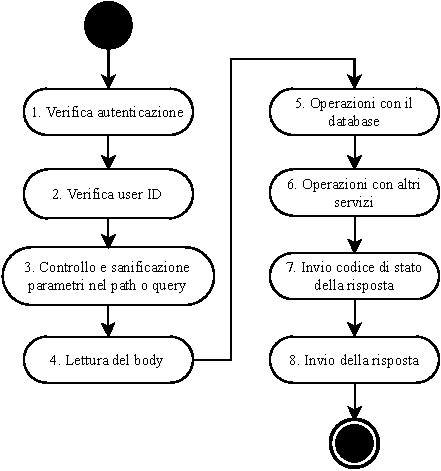
\includegraphics[width=0.7\textwidth]{assets/04/operazioni-api.pdf}
\caption{Passi operativi della gestione di una richiesta per una API.}
\label{fig:operazioni-api}
\end{figure}

L'implementazione di \texttt{GET /chats/\{chatid\}/messages/} viene mostrata come esempio nel listato di codice \ref{listing:impl_api}. Per compattezza il codice relativo alla gestione degli errori è stato nascosto tranne che nel primo caso. Infatti è interessante notare una peculiarità del linguaggio: Go non ha un sistema di eccezioni, la gestione degli errori è esplicita in modo simile al C. Scrivere codice in Go richiede perciò di gestire ogni caso di errore, e il linguaggio aiuta in ciò permettendo la restituzione di più valori da una funzione. A ogni percorso di errore viene stampato un messaggio di log e restituito un codice di errore al client.

Nelle ultime righe di codice è possibile notare come viene creata la risposta: la variabile \texttt{messages} consiste in una sequenza di messaggi e viene convertita in rappresentazione JSON. Tale rappresentazione viene scritta direttamente nel body della risposta, in automatico viene impostato il codice di stato \texttt{200}.

Oltre alla funzione mostrata, c'è parte di codice relativo alla costruzione dei parametri passati nella funzione, la verifica del token di autenticazione, che contiene anche l'user ID, e vario altro codice relativo al sistema in generale.

\begin{longlisting}
\begin{minted}{go}
func (rt *_router) getMessages(w http.ResponseWriter, r *http.Request, ps httprouter.Params, ctx reqcontext.RequestContext) {
	if ctx.UserID == uuid.Nil {
		ctx.Logger.Info("getChats: userid nil")
		w.WriteHeader(http.StatusBadRequest)
		return
	}

	chatid, err := strconv.ParseUint(ps.ByName("chatid"), 10, 64)
	if err != nil {
		// ...
	}

	var fromid uint64
	if rawFromid := r.URL.Query().Get("fromID"); rawFromid != "" {
		var err error
		if fromid, err = strconv.ParseUint(rawFromid, 10, 64); err != nil {
		    // ...
		}
	}

	if _, err = rt.DB.GetUsername(ctx.UserID); err != nil {
		// ...
	}

	messages, err := rt.DB.GetLatestMessages(chatid, fromid)
	if err != nil {
		// ...
	}

	w.Header().Set("content-type", "application/json")
	if err := json.NewEncoder(w).Encode(messages); err != nil {
		// ...
	}
}
\end{minted}
\caption{Implementazione di \texttt{GET /chats/\{chatid\}/messages/}.}
\label{listing:impl_api}
\end{longlisting}

\paragraph{Implementazione per package \texttt{database}} Nel codice mostrato in precedenza è possibile notare che durante la gestione vengono effettuate delle operazioni sul database tramite i metodi \texttt{GetUsername} e \texttt{GetLatestMessages}. Questi metodi contengono la logica per interagire con il database, principalmente la query SQL che viene eseguita, come mostrato nel listato di codice \ref{listing:impl_db} che implementa \texttt{GetLatestMessages}.

La query SQL è costruita in modo di mappare i nomi delle colonne con quelli della struttura \texttt{types.APIMessage}, perché, grazie alla riflessione (indicata anche come \textit{reflection}) di Go, è possibile effettuare una conversione automatica dai tipi del database con quelli della struttura. Il vantaggio di tale uso è la semplicità di scrittura del codice, a costo di una leggera penalità in prestazioni causate dalla riflessione.

\begin{longlisting}
\begin{minted}{go}
func (db *appdbimpl) GetLatestMessages(chatid uint64, fromid uint64) ([]types.APIMessage, error) {
	const (
		queryMessages = `
		SELECT message.id AS id,
			message.createdat AS createdat,
			user.name AS sentby,
			message.type AS type,
			IF(message.type = 'text', message.textcontent, "") AS text,
			IF(message.type = 'slider', message.intcontent, 0) AS slider,
			IF(message.type = 'image', message.textcontent, "") AS image
		FROM message JOIN user ON message.senderid = user.id
		WHERE (chatid = ?) AND (? = 0 OR message.id < ?)
		ORDER BY createdat DESC, id DESC
		LIMIT 25
		`
		queryMessage = `SELECT id FROM message WHERE id = ?`
	)

	// Controllo dell'esistenza di chatid e fromid...

	var latestMessages []types.APIMessage
	if err = db.c.Select(&latestMessages, queryMessages, chatid, fromid, fromid); err != nil {
		return nil, err
	}

	return latestMessages, nil
}
\end{minted}
\caption{Implementazione \texttt{GetLatestMessages}.}
\label{listing:impl_db}
\end{longlisting}

\section{Implementazione nel Worker}

Il Worker nella sostanza è una programma che lancia dei lavori periodici, anche chiamati \textit{task}. Sfrutta molto la concorrenza con le goroutine, infatti quello che fa è avviare dei timer, indipendenti l'uno dall'altro, a cui è associato un task. I timer ogni volta che scattano avviano il task in una nuova goroutine. Il funzionamento è schematizzato nella figura \ref{fig:ciclo_worker}. Sono due i task implementati per la funzionalità delle chat:

\begin{itemize}
\item \texttt{closeChats}: task eseguito in ogni minuto che si occupa di chiudere le chat che non sono state associate ad alcun terremoto entro un tempo arbitrario, per il momento deciso a 24 ore;
\item \texttt{matchChats}: task eseguito in ogni minuto che si occupa di assegnare un terremoto a una chat, in base alla posizione geografica e al tempo di creazione, confrontando gli ultimi terremoti con i dati delle chat.
\end{itemize}

\afterpage{\clearpage}

\begin{figure}[ht!]
\centering
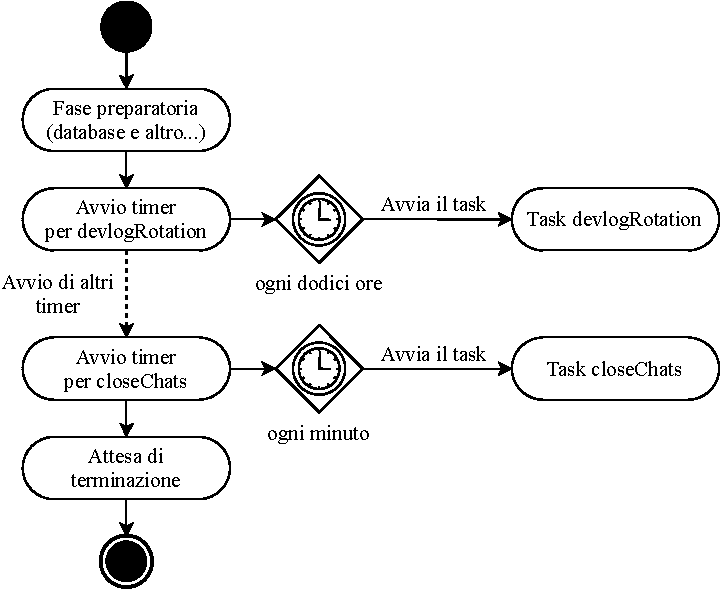
\includegraphics[width=0.85\textwidth]{assets/04/ciclo_vita_worker.pdf}
\caption{Ciclo di vita del Worker.}
\label{fig:ciclo_worker}
\end{figure}

Viene portato come esempio l'implementazione del task \texttt{closeChats} nel listato di codice \ref{listing:impl_worker}. In questo caso consiste soltanto di una query SQL di aggiornamento.

\begin{longlisting}
\begin{minted}{go}
func (w *_worker) closeChats() {
	const query = `
	UPDATE chat
	SET closed = TRUE
	WHERE closed = FALSE AND earthquakeid IS NULL AND createdat < NOW() - INTERVAL 24 HOUR
	`

	res, err := w.db.Exec(query)
	if err != nil {
		// ...
	}
	
	// Codice di log...
}
\end{minted}
\caption{Implementazione del task \texttt{closeChats} in Worker.}
\label{listing:impl_worker}
\end{longlisting}

\section{Test}

Durante l'implementazione delle API e dei task nel Worker sono state effettuate diverse prove manuali nell'ambiente di sviluppo locale. Dei vari tipi di test possibili, si sono preferiti quelli di integrazione per provare le API, verificando i risultati nel database o nelle risposte HTTP. In un secondo momento si è tentato di automatizzare in modo parziale i test tramite un programma scritto in Go che effettua le richieste e controlla la risposta per tutte le API. Il listato di codice \ref{listing:impl_test} mostra la funzione \texttt{TestPutUsername} che verifica i possibili codici di stato ritornati dall'API \texttt{PUT /me/username}. La funzione \texttt{testPutUsername} costruisce e invia la richiesta HTTP, poi verificare il codice di stato con quello passato come argomento.

La soluzione costruita non è risultata del tutto soddisfacente: per poter lanciare il programma di test è necessario configurare manualmente il servizio di autenticazione Keycloak, inoltre il database deve essere riportato allo stato originario dopo ogni esecuzione.

\begin{longlisting}
\begin{minted}{go}
func TestPutUsername(t *testing.T) {
	t.Run("200-OK", func(t *testing.T) {
		testPutUsername(t, "Giampiero", http.StatusOK)
	})
	t.Run("400-TOO-SHORT", func(t *testing.T) {
		testPutUsername(t, "Gi", http.StatusBadRequest)
	})
	t.Run("400-EMPTY-BODY", func(t *testing.T) {
		testPutUsername(t, "", http.StatusBadRequest)
	})
	t.Run("400-TOO-LONG", func(t *testing.T) {
		testPutUsername(t, "usernamemoltomoltomoltomoltolungo...", http.StatusBadRequest)
	})
}
\end{minted}
\caption{Esempio di test per \texttt{PUT /me/username}.}
\label{listing:impl_test}
\end{longlisting}